\documentclass{article}
\usepackage{tabularx}
\usepackage{amsmath}
\usepackage{graphicx}
\usepackage[margin=2cm]{geometry}
\usepackage{cite}
\usepackage[final]{hyperref}
\usepackage{listings}
\hypersetup{
	colorlinks=true,
	linkcolor=blue,
	citecolor=blue,
	filecolor=magenta,
	urlcolor=blue         
}

\begin{document}

\title{Practicle 1\\Introduction to CUDA}
\author{Robin Faury}
\date{19/12/18}
\maketitle

\begin{abstract}
	In this practical work, we will see how to convert a simple iterative process into a paralell process using CUDA language. This is a quick and simple introduction du CUDA. The aim is just to understand the syntax and how to store and access buffers in the GPU memory. You have to write a quick report for the 9th of January 2019.
\end{abstract}


\section{Introduction}
First, generate the Visual Studio solution, compile it and run the helloworld cuda program.
You'll find the source of the practicle work by cloning this git repository:
\begin{lstlisting}
	https://github.com/robinfaurypro/cuda\_lessons.git
\end{lstlisting}
The CMakeLists file is stored into the practicles folder. Open a terminal on your working folder and use this cmake command:
\begin{lstlisting}
	cmake -G "Visual Studio 15 Win64" ..
\end{lstlisting}
If everything is going well, you can compile and run the cuda\_lesson\_helloworld executable.\\
Using MSVC compiler for Visual Studio IDE is not the only option. You can also use the CUDA C++ compiler via the terminal. 
\begin{lstlisting}
	nvcc main.cu -o cuda_lesson_helloworld
\end{lstlisting}
The cuda file extention is .cu.

\section{The host}
Remember the host is the CPU part of the process. So you have to declare and fill input buffers before the GPU copy. For this exemple we will use the GPU to encrypt a text using the Caesar cipher. It is the simplest encryption technique. Each character is shifted to the right by x.

\begin{figure}[h]
	\centering
	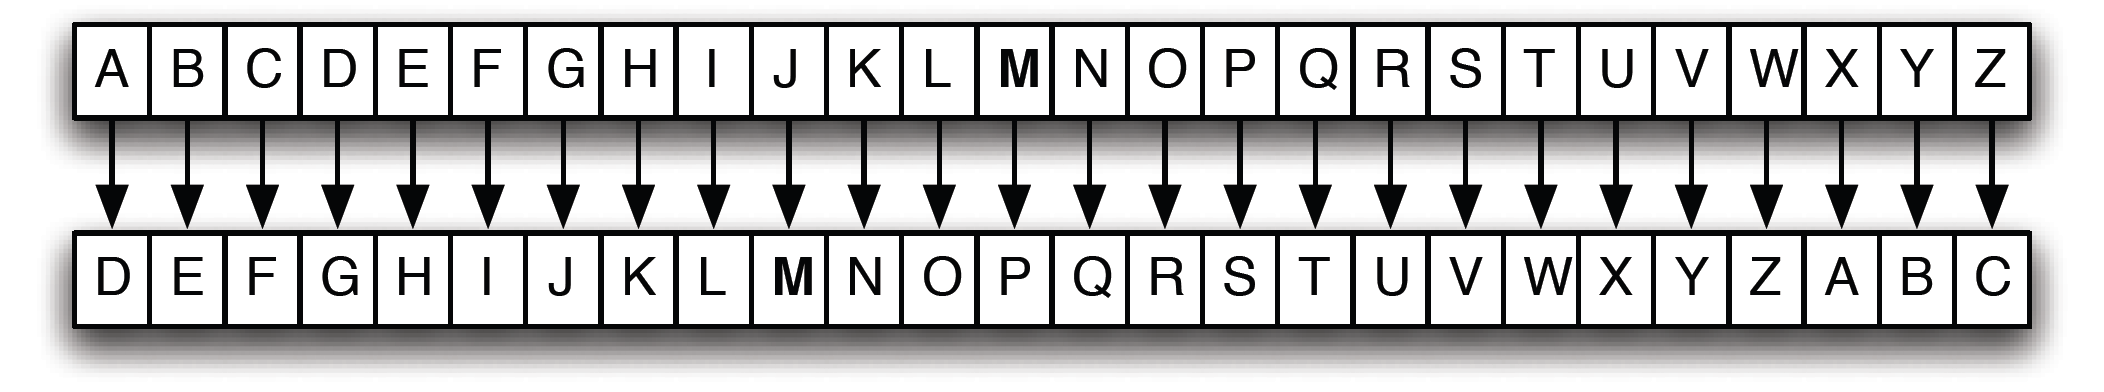
\includegraphics[scale=0.25]{figures/caesar.png}
	\caption{Caesar cipher}
\end{figure}

First we have to create a buffer of char for the input buffer and another with the same size for the output result. You can hardcode the input or pass it as a program argument or use an external file. For this first exercice we will use Test-Driven Development (TDD). The aim is to write all the fonctional and unit tests before developing the feature. Thinking about corner cases before creating the tool is the best way to avoid bugs.
Write some useful tests, for exemple:
\begin{itemize}
	\item no corrupted data
	\item a sting encrypted by x and -x is the same
	\item ...
\end{itemize}
At this stage, all your tests must fail.

\section{The device}
The device is related to GPU operations. On this section, we will see how to send buffers to the VRAM and declare and run kernels. 
\subsection{The memory}
	Before doing the copy to the CUDA's Unified Memory from the host we must allocate the space. The function cudaMallocManaged takes as input a pointer and the data size. Remember that the N value will be spread into warps (a block of 32 threads). It should be a multiple of 32.
\begin{lstlisting}
	char* buffer;
	cudaMallocManaged(&buffer, N*sizeof(char));
\end{lstlisting}
	As usual, you must delete your pointer. For this use this cuda function:
\begin{lstlisting}
	cudaFree(buffer);
\end{lstlisting}

\subsection{The kernel}
	Declaring a kernel is easy with CUDA. You just have to write your code like a C++ function and add the \_\_global\_\_ keyword before. This indicates the CUDA C++ compiler that your function is device code. 
\begin{lstlisting}
	__global__
	void caesarEncode(int bufferSize, char *buffer, char *outBuffer, int shiftValue)
	{
		for (unsigned int i = 0u; i < bufferSize; i++)
			outBuffer[i] = buffer[i] + shiftValue;
	}
\end{lstlisting}
For the moment the function is designed for one thread. We can run this function using this syntaxe:
\begin{lstlisting}
	// We use one thread per block and one block per grid
	caesarEncode<<<1, 1>>>(bufferSize, buffer, outBuffer, 10);
\end{lstlisting}
Let's increment the number of threads per block. Something like 256 may a good value for big buffers. CUDA allows us to know the index of the thread through the threadIdx.x value. 

\begin{lstlisting}
	__global__
	void caesarEncode(int bufferSize, char *buffer, char *outBuffer, int shiftValue)
	{
		int stride = blockDim.x; // stride = 256
		int index = threadIdx.x;
		for (int i = index; i < bufferSize; i += stride)
			outBuffer[i] = buffer[i] + shiftValue;
	}
	
	// ...

	// We use 256 threads per block and one block per grid
	caesarEncode<<<1, 256>>>(bufferSize, buffer, outBuffer, 10);
\end{lstlisting}

In the same way we can increase the number of blocks per grid to dispatch the computation on every streaming multiprocessor.
\begin{lstlisting}
	__global__
	void caesarEncode(int bufferSize, char *buffer, char *outBuffer, int shiftValue)
	{
		int stride = blockDim.x * gridDim.x; // stride = 256 * blockPerGrid
		int index = blockIdx.x * blockDim.x + threadIdx.x;
		for (int i = index; i < bufferSize; i += stride)
			outBuffer[i] = buffer[i] + shiftValue;
	}
	
	// ...

	// We use 256 threads per block and one block per grid
	int blockPerGrid = (N + 256 - 1) / blockSize;
	caesarEncode<<<blockPerGrid, 256>>>(bufferSize, buffer, outBuffer, 10);
\end{lstlisting}
We can notice in this case that we run N threads so we can remove the for loop.

\section{result}
If everything is going well "HELLO WORLD" should become "KHOOR ZRUOG" for a shift value of 3.

\subsection{Profiling}
The execution speed can be evaluated using an Nvidia tool. Open a terminal from your executable folder and run it using nvprof
\begin{lstlisting}
	nvprof ./cuda_lessons_practicle01.exe
\end{lstlisting}
This tool shows you the time spent by the caesarEncode function. Make a few tests comparing timing for some values of N, threads per block and blocks per grid.

\section{Going forward}
We can notice threadIdx.x has a 'x' struct member. That means we can organize our threads per blocks (even blocks per grid) in a non linear way using the CUDA object dim3.
\begin{lstlisting}
	__global__
	void matrixMul(float *matrixA16x16, float *matrixB16x16, float *outMatrix16x16)
	{
		int i = blockIdx.x * blockDim.x + threadIdx.x;
		int j = blockIdx.y * blockDim.y + threadIdx.y;
		// ...
	}

	// ...

	dim3 threadsPerBlock(16, 16);
	// We use 256 threads per block and one block per grid
	matrixMul<<<1, threadsPerBlock>>>(matrixA16x16, matrixB16x16, outMatrix16x16);
\end{lstlisting}
\end{document}